\documentclass[twoside]{book}

% Packages required by doxygen
\usepackage{fixltx2e}
\usepackage{calc}
\usepackage{doxygen}
\usepackage[export]{adjustbox} % also loads graphicx
\usepackage{graphicx}
\usepackage[utf8]{inputenc}
\usepackage{makeidx}
\usepackage{multicol}
\usepackage{multirow}
\PassOptionsToPackage{warn}{textcomp}
\usepackage{textcomp}
\usepackage[nointegrals]{wasysym}
\usepackage[table]{xcolor}

% Font selection
\usepackage[T1]{fontenc}
\usepackage[scaled=.90]{helvet}
\usepackage{courier}
\usepackage{amssymb}
\usepackage{sectsty}
\renewcommand{\familydefault}{\sfdefault}
\allsectionsfont{%
  \fontseries{bc}\selectfont%
  \color{darkgray}%
}
\renewcommand{\DoxyLabelFont}{%
  \fontseries{bc}\selectfont%
  \color{darkgray}%
}
\newcommand{\+}{\discretionary{\mbox{\scriptsize$\hookleftarrow$}}{}{}}

% Page & text layout
\usepackage{geometry}
\geometry{%
  a4paper,%
  top=2.5cm,%
  bottom=2.5cm,%
  left=2.5cm,%
  right=2.5cm%
}
\tolerance=750
\hfuzz=15pt
\hbadness=750
\setlength{\emergencystretch}{15pt}
\setlength{\parindent}{0cm}
\setlength{\parskip}{3ex plus 2ex minus 2ex}
\makeatletter
\renewcommand{\paragraph}{%
  \@startsection{paragraph}{4}{0ex}{-1.0ex}{1.0ex}{%
    \normalfont\normalsize\bfseries\SS@parafont%
  }%
}
\renewcommand{\subparagraph}{%
  \@startsection{subparagraph}{5}{0ex}{-1.0ex}{1.0ex}{%
    \normalfont\normalsize\bfseries\SS@subparafont%
  }%
}
\makeatother

% Headers & footers
\usepackage{fancyhdr}
\pagestyle{fancyplain}
\fancyhead[LE]{\fancyplain{}{\bfseries\thepage}}
\fancyhead[CE]{\fancyplain{}{}}
\fancyhead[RE]{\fancyplain{}{\bfseries\leftmark}}
\fancyhead[LO]{\fancyplain{}{\bfseries\rightmark}}
\fancyhead[CO]{\fancyplain{}{}}
\fancyhead[RO]{\fancyplain{}{\bfseries\thepage}}
\fancyfoot[LE]{\fancyplain{}{}}
\fancyfoot[CE]{\fancyplain{}{}}
\fancyfoot[RE]{\fancyplain{}{\bfseries\scriptsize Generated by Doxygen }}
\fancyfoot[LO]{\fancyplain{}{\bfseries\scriptsize Generated by Doxygen }}
\fancyfoot[CO]{\fancyplain{}{}}
\fancyfoot[RO]{\fancyplain{}{}}
\renewcommand{\footrulewidth}{0.4pt}
\renewcommand{\chaptermark}[1]{%
  \markboth{#1}{}%
}
\renewcommand{\sectionmark}[1]{%
  \markright{\thesection\ #1}%
}

% Indices & bibliography
\usepackage{natbib}
\usepackage[titles]{tocloft}
\setcounter{tocdepth}{3}
\setcounter{secnumdepth}{5}
\makeindex

% Hyperlinks (required, but should be loaded last)
\usepackage{ifpdf}
\ifpdf
  \usepackage[pdftex,pagebackref=true]{hyperref}
\else
  \usepackage[ps2pdf,pagebackref=true]{hyperref}
\fi
\hypersetup{%
  colorlinks=true,%
  linkcolor=blue,%
  citecolor=blue,%
  unicode%
}

% Custom commands
\newcommand{\clearemptydoublepage}{%
  \newpage{\pagestyle{empty}\cleardoublepage}%
}

\usepackage{caption}
\captionsetup{labelsep=space,justification=centering,font={bf},singlelinecheck=off,skip=4pt,position=top}

%===== C O N T E N T S =====

\begin{document}

% Titlepage & ToC
\hypersetup{pageanchor=false,
             bookmarksnumbered=true,
             pdfencoding=unicode
            }
\pagenumbering{alph}
\begin{titlepage}
\vspace*{7cm}
\begin{center}%
{\Large My Project }\\
\vspace*{1cm}
{\large Generated by Doxygen 1.8.13}\\
\end{center}
\end{titlepage}
\clearemptydoublepage
\pagenumbering{roman}
\tableofcontents
\clearemptydoublepage
\pagenumbering{arabic}
\hypersetup{pageanchor=true}

%--- Begin generated contents ---
\chapter{Essay Generator}
\label{index}\hypertarget{index}{}\hypertarget{index_Introduction}{}\section{Introduction}\label{index_Introduction}
Write an English essay on a given topic, provided with a set of source documents.\hypertarget{index_Authors}{}\section{Authors}\label{index_Authors}
40014082 Ling Tan ~\newline
40018813 Rui Zhao ~\newline
27419694 Vincent Boivin 
\chapter{Hierarchical Index}
\section{Class Hierarchy}
This inheritance list is sorted roughly, but not completely, alphabetically\+:\begin{DoxyCompactList}
\item \contentsline{section}{Abstract\+Tokenizer}{\pageref{classAbstractTokenizer}}{}
\begin{DoxyCompactList}
\item \contentsline{section}{Sentence\+Tokenizer}{\pageref{classSentenceTokenizer}}{}
\item \contentsline{section}{Word\+Tokenizer}{\pageref{classWordTokenizer}}{}
\end{DoxyCompactList}
\item \contentsline{section}{Indexer}{\pageref{classIndexer}}{}
\begin{DoxyCompactList}
\item \contentsline{section}{Document\+Indexer}{\pageref{classDocumentIndexer}}{}
\item \contentsline{section}{Sentence\+Indexer}{\pageref{classSentenceIndexer}}{}
\end{DoxyCompactList}
\item \contentsline{section}{Index\+Item}{\pageref{classIndexItem}}{}
\begin{DoxyCompactList}
\item \contentsline{section}{Document}{\pageref{classDocument}}{}
\item \contentsline{section}{Sentence}{\pageref{classSentence}}{}
\end{DoxyCompactList}
\item \contentsline{section}{Query\+Result}{\pageref{classQueryResult}}{}
\item \contentsline{section}{Stopword}{\pageref{classStopword}}{}
\end{DoxyCompactList}

\chapter{Class Index}
\section{Class List}
Here are the classes, structs, unions and interfaces with brief descriptions\+:\begin{DoxyCompactList}
\item\contentsline{section}{\hyperlink{classAbstractTokenizer}{Abstract\+Tokenizer} }{\pageref{classAbstractTokenizer}}{}
\item\contentsline{section}{\hyperlink{classDocument}{Document} }{\pageref{classDocument}}{}
\item\contentsline{section}{\hyperlink{classDocumentIndexer}{Document\+Indexer} }{\pageref{classDocumentIndexer}}{}
\item\contentsline{section}{\hyperlink{classIndexer}{Indexer} }{\pageref{classIndexer}}{}
\item\contentsline{section}{\hyperlink{classIndexItem}{Index\+Item} }{\pageref{classIndexItem}}{}
\item\contentsline{section}{\hyperlink{classQueryResult}{Query\+Result} }{\pageref{classQueryResult}}{}
\item\contentsline{section}{\hyperlink{classSentence}{Sentence} }{\pageref{classSentence}}{}
\item\contentsline{section}{\hyperlink{classSentenceIndexer}{Sentence\+Indexer} }{\pageref{classSentenceIndexer}}{}
\item\contentsline{section}{\hyperlink{classSentenceTokenizer}{Sentence\+Tokenizer} }{\pageref{classSentenceTokenizer}}{}
\item\contentsline{section}{\hyperlink{classStopword}{Stopword} }{\pageref{classStopword}}{}
\item\contentsline{section}{\hyperlink{classWordTokenizer}{Word\+Tokenizer} }{\pageref{classWordTokenizer}}{}
\end{DoxyCompactList}

\chapter{Class Documentation}
\hypertarget{classAbstractTokenizer}{}\section{Abstract\+Tokenizer Class Reference}
\label{classAbstractTokenizer}\index{Abstract\+Tokenizer@{Abstract\+Tokenizer}}


Inheritance diagram for Abstract\+Tokenizer\+:\nopagebreak
\begin{figure}[H]
\begin{center}
\leavevmode
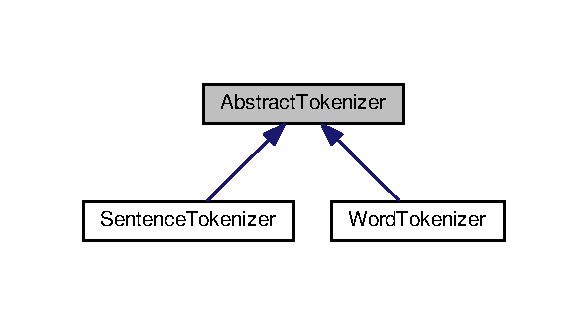
\includegraphics[width=282pt]{classAbstractTokenizer__inherit__graph}
\end{center}
\end{figure}
\subsection*{Public Member Functions}
\begin{DoxyCompactItemize}
\item 
\hyperlink{classAbstractTokenizer_ad5dd529f11552a1bb522f97077148270}{Abstract\+Tokenizer} ()
\item 
virtual \hyperlink{classAbstractTokenizer_ac9005dbf8971809768ddfeea2db3e3a9}{$\sim$\+Abstract\+Tokenizer} ()
\item 
const std\+::vector$<$ std\+::string $>$ \& \hyperlink{classAbstractTokenizer_a1c23c57444bf8356347f1ae113034d1b}{get\+Tokens} () const
\item 
const size\+\_\+t \hyperlink{classAbstractTokenizer_ab1f0ec877a204abe9338f290e515e7d7}{get\+Size} () const
\end{DoxyCompactItemize}
\subsection*{Protected Attributes}
\begin{DoxyCompactItemize}
\item 
std\+::vector$<$ std\+::string $>$ \hyperlink{classAbstractTokenizer_a76c3d1105c591f92f1036c327acd36f3}{tokens}
\item 
size\+\_\+t \hyperlink{classAbstractTokenizer_a25d4d9be114e714ac362dd64991e0f65}{size}
\end{DoxyCompactItemize}
\subsection*{Friends}
\begin{DoxyCompactItemize}
\item 
std\+::ostream \& \hyperlink{classAbstractTokenizer_afe537fa967b2a1d1db799e201b4007fa}{operator$<$$<$} (std\+::ostream \&, const \hyperlink{classAbstractTokenizer}{Abstract\+Tokenizer} \&)
\end{DoxyCompactItemize}


\subsection{Constructor \& Destructor Documentation}
\mbox{\Hypertarget{classAbstractTokenizer_ad5dd529f11552a1bb522f97077148270}\label{classAbstractTokenizer_ad5dd529f11552a1bb522f97077148270}} 
\index{Abstract\+Tokenizer@{Abstract\+Tokenizer}!Abstract\+Tokenizer@{Abstract\+Tokenizer}}
\index{Abstract\+Tokenizer@{Abstract\+Tokenizer}!Abstract\+Tokenizer@{Abstract\+Tokenizer}}
\subsubsection{\texorpdfstring{Abstract\+Tokenizer()}{AbstractTokenizer()}}
{\footnotesize\ttfamily Abstract\+Tokenizer\+::\+Abstract\+Tokenizer (\begin{DoxyParamCaption}{ }\end{DoxyParamCaption})}

Default constructor \mbox{\Hypertarget{classAbstractTokenizer_ac9005dbf8971809768ddfeea2db3e3a9}\label{classAbstractTokenizer_ac9005dbf8971809768ddfeea2db3e3a9}} 
\index{Abstract\+Tokenizer@{Abstract\+Tokenizer}!````~Abstract\+Tokenizer@{$\sim$\+Abstract\+Tokenizer}}
\index{````~Abstract\+Tokenizer@{$\sim$\+Abstract\+Tokenizer}!Abstract\+Tokenizer@{Abstract\+Tokenizer}}
\subsubsection{\texorpdfstring{$\sim$\+Abstract\+Tokenizer()}{~AbstractTokenizer()}}
{\footnotesize\ttfamily Abstract\+Tokenizer\+::$\sim$\+Abstract\+Tokenizer (\begin{DoxyParamCaption}{ }\end{DoxyParamCaption})\hspace{0.3cm}{\ttfamily [virtual]}}

Default destructor 

\subsection{Member Function Documentation}
\mbox{\Hypertarget{classAbstractTokenizer_ab1f0ec877a204abe9338f290e515e7d7}\label{classAbstractTokenizer_ab1f0ec877a204abe9338f290e515e7d7}} 
\index{Abstract\+Tokenizer@{Abstract\+Tokenizer}!get\+Size@{get\+Size}}
\index{get\+Size@{get\+Size}!Abstract\+Tokenizer@{Abstract\+Tokenizer}}
\subsubsection{\texorpdfstring{get\+Size()}{getSize()}}
{\footnotesize\ttfamily const size\+\_\+t Abstract\+Tokenizer\+::get\+Size (\begin{DoxyParamCaption}{ }\end{DoxyParamCaption}) const}

Get the number of tokens \begin{DoxyReturn}{Returns}

\end{DoxyReturn}
\mbox{\Hypertarget{classAbstractTokenizer_a1c23c57444bf8356347f1ae113034d1b}\label{classAbstractTokenizer_a1c23c57444bf8356347f1ae113034d1b}} 
\index{Abstract\+Tokenizer@{Abstract\+Tokenizer}!get\+Tokens@{get\+Tokens}}
\index{get\+Tokens@{get\+Tokens}!Abstract\+Tokenizer@{Abstract\+Tokenizer}}
\subsubsection{\texorpdfstring{get\+Tokens()}{getTokens()}}
{\footnotesize\ttfamily const std\+::vector$<$ std\+::string $>$ \& Abstract\+Tokenizer\+::get\+Tokens (\begin{DoxyParamCaption}{ }\end{DoxyParamCaption}) const}

Get tokens \begin{DoxyReturn}{Returns}

\end{DoxyReturn}


\subsection{Friends And Related Function Documentation}
\mbox{\Hypertarget{classAbstractTokenizer_afe537fa967b2a1d1db799e201b4007fa}\label{classAbstractTokenizer_afe537fa967b2a1d1db799e201b4007fa}} 
\index{Abstract\+Tokenizer@{Abstract\+Tokenizer}!operator$<$$<$@{operator$<$$<$}}
\index{operator$<$$<$@{operator$<$$<$}!Abstract\+Tokenizer@{Abstract\+Tokenizer}}
\subsubsection{\texorpdfstring{operator$<$$<$}{operator<<}}
{\footnotesize\ttfamily std\+::ostream\& operator$<$$<$ (\begin{DoxyParamCaption}\item[{std\+::ostream \&}]{,  }\item[{const \hyperlink{classAbstractTokenizer}{Abstract\+Tokenizer} \&}]{ }\end{DoxyParamCaption})\hspace{0.3cm}{\ttfamily [friend]}}

output \hyperlink{classAbstractTokenizer}{Abstract\+Tokenizer} \begin{DoxyReturn}{Returns}

\end{DoxyReturn}


\subsection{Member Data Documentation}
\mbox{\Hypertarget{classAbstractTokenizer_a25d4d9be114e714ac362dd64991e0f65}\label{classAbstractTokenizer_a25d4d9be114e714ac362dd64991e0f65}} 
\index{Abstract\+Tokenizer@{Abstract\+Tokenizer}!size@{size}}
\index{size@{size}!Abstract\+Tokenizer@{Abstract\+Tokenizer}}
\subsubsection{\texorpdfstring{size}{size}}
{\footnotesize\ttfamily size\+\_\+t Abstract\+Tokenizer\+::size\hspace{0.3cm}{\ttfamily [protected]}}

number of tokens \mbox{\Hypertarget{classAbstractTokenizer_a76c3d1105c591f92f1036c327acd36f3}\label{classAbstractTokenizer_a76c3d1105c591f92f1036c327acd36f3}} 
\index{Abstract\+Tokenizer@{Abstract\+Tokenizer}!tokens@{tokens}}
\index{tokens@{tokens}!Abstract\+Tokenizer@{Abstract\+Tokenizer}}
\subsubsection{\texorpdfstring{tokens}{tokens}}
{\footnotesize\ttfamily std\+::vector$<$std\+::string$>$ Abstract\+Tokenizer\+::tokens\hspace{0.3cm}{\ttfamily [protected]}}

token vector 

The documentation for this class was generated from the following files\+:\begin{DoxyCompactItemize}
\item 
headers/Abstract\+Tokenizer.\+h\item 
implementation/Abstract\+Tokenizer.\+cpp\end{DoxyCompactItemize}

\hypertarget{classDocument}{\section{Document Class Reference}
\label{classDocument}\index{Document@{Document}}
}


{\ttfamily \#include $<$Document.\-h$>$}

Inheritance diagram for Document\-:\begin{figure}[H]
\begin{center}
\leavevmode
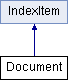
\includegraphics[height=2.000000cm]{classDocument}
\end{center}
\end{figure}
\subsection*{Public Member Functions}
\begin{DoxyCompactItemize}
\item 
\hyperlink{classDocument_acdbcbe550084e8c20f4f67eb229ad66a}{Document} ()
\item 
\hyperlink{classDocument_a11e577354c64a23106b0cf34c11e712f}{Document} (const std\-::string \&file\-Name)
\item 
const void \hyperlink{classDocument_a9c9a23f1b4651aff6b885c2a69bc76d2}{tokenize\-By\-Content} (const std\-::string \&file\-Name, const std\-::string \&content)
\item 
const std\-::size\-\_\-t \hyperlink{classDocument_ab93c5c78b8d8b2fb6f9a2739d4c967ca}{get\-Size} () const overridefinal
\end{DoxyCompactItemize}
\subsection*{Friends}
\begin{DoxyCompactItemize}
\item 
\hypertarget{classDocument_a801e6c851261e550881c632d31407c55}{std\-::ostream \& {\bfseries operator$<$$<$} (std\-::ostream \&, const \hyperlink{classDocument}{Document} \&)}\label{classDocument_a801e6c851261e550881c632d31407c55}

\end{DoxyCompactItemize}
\subsection*{Additional Inherited Members}


\subsection{Detailed Description}
A document object d represents one document in your index.\textbackslash{} It provides a default constructor,which creates an empty document, a constructor that accepts a file name and reads the file contents into the document object. Each document provides the functions name() (returns the file name of the document), size() (size in characters), content() (returns the text of the document). 

\subsection{Constructor \& Destructor Documentation}
\hypertarget{classDocument_acdbcbe550084e8c20f4f67eb229ad66a}{\index{Document@{Document}!Document@{Document}}
\index{Document@{Document}!Document@{Document}}
\subsubsection[{Document}]{\setlength{\rightskip}{0pt plus 5cm}Document\-::\-Document (
\begin{DoxyParamCaption}
{}
\end{DoxyParamCaption}
)}}\label{classDocument_acdbcbe550084e8c20f4f67eb229ad66a}
Default constructor \hypertarget{classDocument_a11e577354c64a23106b0cf34c11e712f}{\index{Document@{Document}!Document@{Document}}
\index{Document@{Document}!Document@{Document}}
\subsubsection[{Document}]{\setlength{\rightskip}{0pt plus 5cm}Document\-::\-Document (
\begin{DoxyParamCaption}
\item[{const std\-::string \&}]{file\-Name}
\end{DoxyParamCaption}
)}}\label{classDocument_a11e577354c64a23106b0cf34c11e712f}
Constructor accepts a file name and reads the file contents into the document object 
\begin{DoxyParams}{Parameters}
{\em file\-Name} & \\
\hline
\end{DoxyParams}
!! size is in characters !!!// 

\subsection{Member Function Documentation}
\hypertarget{classDocument_ab93c5c78b8d8b2fb6f9a2739d4c967ca}{\index{Document@{Document}!get\-Size@{get\-Size}}
\index{get\-Size@{get\-Size}!Document@{Document}}
\subsubsection[{get\-Size}]{\setlength{\rightskip}{0pt plus 5cm}const size\-\_\-t Document\-::get\-Size (
\begin{DoxyParamCaption}
{}
\end{DoxyParamCaption}
) const\hspace{0.3cm}{\ttfamily [final]}, {\ttfamily [override]}, {\ttfamily [virtual]}}}\label{classDocument_ab93c5c78b8d8b2fb6f9a2739d4c967ca}
Get document size \begin{DoxyReturn}{Returns}
the size of document 
\end{DoxyReturn}


Reimplemented from \hyperlink{classIndexItem_a96cbdc874ef50fd1f51bf39d526cabf8}{Index\-Item}.

\hypertarget{classDocument_a9c9a23f1b4651aff6b885c2a69bc76d2}{\index{Document@{Document}!tokenize\-By\-Content@{tokenize\-By\-Content}}
\index{tokenize\-By\-Content@{tokenize\-By\-Content}!Document@{Document}}
\subsubsection[{tokenize\-By\-Content}]{\setlength{\rightskip}{0pt plus 5cm}const void Document\-::tokenize\-By\-Content (
\begin{DoxyParamCaption}
\item[{const std\-::string \&}]{file\-Name, }
\item[{const std\-::string \&}]{content}
\end{DoxyParamCaption}
)}}\label{classDocument_a9c9a23f1b4651aff6b885c2a69bc76d2}
Tokenizer a file by giving file name and its content 
\begin{DoxyParams}{Parameters}
{\em file\-Name} & \\
\hline
{\em content} & \\
\hline
\end{DoxyParams}
!! size is in wrods !!!// 

The documentation for this class was generated from the following files\-:\begin{DoxyCompactItemize}
\item 
headers/Document.\-h\item 
implementation/Document.\-cpp\end{DoxyCompactItemize}

\hypertarget{classDocumentIndexer}{\section{Document\-Indexer Class Reference}
\label{classDocumentIndexer}\index{Document\-Indexer@{Document\-Indexer}}
}
Inheritance diagram for Document\-Indexer\-:\begin{figure}[H]
\begin{center}
\leavevmode
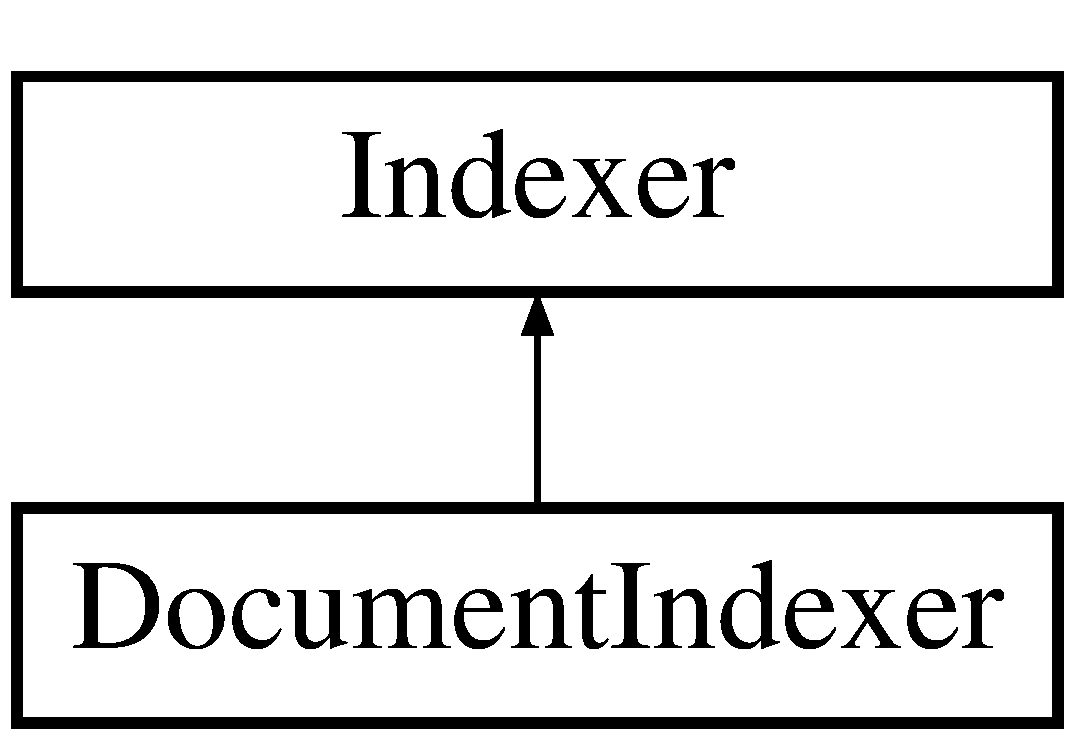
\includegraphics[height=2.000000cm]{classDocumentIndexer}
\end{center}
\end{figure}
\subsection*{Public Member Functions}
\begin{DoxyCompactItemize}
\item 
\hyperlink{classDocumentIndexer_a44f3c39ee50c32c0226fe98a66f71d07}{Document\-Indexer} ()
\item 
\hyperlink{classDocumentIndexer_aa3b39750a5477caa4aeab84f1c690c20}{$\sim$\-Document\-Indexer} ()
\end{DoxyCompactItemize}
\subsection*{Friends}
\begin{DoxyCompactItemize}
\item 
\hypertarget{classDocumentIndexer_a784b00aedd8ffb46de57ea05792250d8}{std\-::ostream \& {\bfseries operator$<$$<$} (std\-::ostream \&, const \hyperlink{classDocumentIndexer}{Document\-Indexer} \&)}\label{classDocumentIndexer_a784b00aedd8ffb46de57ea05792250d8}

\end{DoxyCompactItemize}
\subsection*{Additional Inherited Members}


\subsection{Constructor \& Destructor Documentation}
\hypertarget{classDocumentIndexer_a44f3c39ee50c32c0226fe98a66f71d07}{\index{Document\-Indexer@{Document\-Indexer}!Document\-Indexer@{Document\-Indexer}}
\index{Document\-Indexer@{Document\-Indexer}!DocumentIndexer@{Document\-Indexer}}
\subsubsection[{Document\-Indexer}]{\setlength{\rightskip}{0pt plus 5cm}Document\-Indexer\-::\-Document\-Indexer (
\begin{DoxyParamCaption}
{}
\end{DoxyParamCaption}
)}}\label{classDocumentIndexer_a44f3c39ee50c32c0226fe98a66f71d07}
Default constructor \hypertarget{classDocumentIndexer_aa3b39750a5477caa4aeab84f1c690c20}{\index{Document\-Indexer@{Document\-Indexer}!$\sim$\-Document\-Indexer@{$\sim$\-Document\-Indexer}}
\index{$\sim$\-Document\-Indexer@{$\sim$\-Document\-Indexer}!DocumentIndexer@{Document\-Indexer}}
\subsubsection[{$\sim$\-Document\-Indexer}]{\setlength{\rightskip}{0pt plus 5cm}Document\-Indexer\-::$\sim$\-Document\-Indexer (
\begin{DoxyParamCaption}
{}
\end{DoxyParamCaption}
)}}\label{classDocumentIndexer_aa3b39750a5477caa4aeab84f1c690c20}
Default destructor 

The documentation for this class was generated from the following files\-:\begin{DoxyCompactItemize}
\item 
headers/Document\-Indexer.\-h\item 
implementation/Document\-Indexer.\-cpp\end{DoxyCompactItemize}

\hypertarget{classIndexer}{\section{Indexer Class Reference}
\label{classIndexer}\index{Indexer@{Indexer}}
}
Inheritance diagram for Indexer\-:\begin{figure}[H]
\begin{center}
\leavevmode
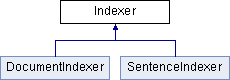
\includegraphics[height=2.000000cm]{classIndexer}
\end{center}
\end{figure}
\subsection*{Public Member Functions}
\begin{DoxyCompactItemize}
\item 
\hyperlink{classIndexer_ac4c8c21c68d62185ceddbad8781e3b67}{Indexer} ()
\item 
virtual \hyperlink{classIndexer_aaf5971639a7a2e3d9af4d8da62deb6f4}{$\sim$\-Indexer} ()
\item 
const long \hyperlink{classIndexer_a55ec44403e327e1720a834f6b7c2289d}{get\-Size} () const 
\item 
const std\-::map$<$ const \\*
std\-::string, unsigned long $>$ \hyperlink{classIndexer_a92be0b09f21160df9e927d76dfbe48d1}{get\-Dictionary} ()
\item 
void \hyperlink{classIndexer_ae090be1899c4ce1e4baeb0acfe12cdee}{normalize} ()
\item 
const double \hyperlink{classIndexer_a646d73e4daefd444e0ab1491e68e5b5e}{get\-Document\-Frequency} (const std\-::string \&t) const 
\item 
const double \hyperlink{classIndexer_ab40a5e7cf5767dea0c6e28ab12b20f60}{get\-Weight} (const std\-::string \&t, const \hyperlink{classIndexItem}{Index\-Item} \&d) const 
\item 
const double \hyperlink{classIndexer_a7eaa5c834d2ea0d87c1de65ce53c74e2}{get\-Weight} (const std\-::string \&t, double tf, const \hyperlink{classIndexItem}{Index\-Item} \&d) const 
\item 
const double \hyperlink{classIndexer_a164449012701532738e578b990fb6dab}{get\-Query\-Weight} (const std\-::string \&t, const \hyperlink{classIndexItem}{Index\-Item} \&d) const 
\item 
virtual const std\-::vector\\*
$<$ \hyperlink{classQueryResult}{Query\-Result} $>$ \hyperlink{classIndexer_abd1dd6a6da0c9e43efaa99866c538e6c}{query} (const std\-::string, const unsigned int=10)
\item 
\hypertarget{classIndexer_aafca8bb21d67052dcf665cdc714db17b}{virtual const std\-::vector\\*
$<$ \hyperlink{classQueryResult}{Query\-Result} $>$ {\bfseries query\-By\-Count} (const std\-::string, const unsigned int=10)}\label{classIndexer_aafca8bb21d67052dcf665cdc714db17b}

\item 
virtual const \hyperlink{classIndexItem}{Index\-Item} $\ast$ \hyperlink{classIndexer_a2f2530920425342d0b4f8652c7368ecd}{operator\mbox{[}$\,$\mbox{]}} (unsigned long) const 
\item 
\hypertarget{classIndexer_a115a9ee696a07c02cadf38e294ce16e4}{const unsigned long {\bfseries search\-Dictionary} (std\-::map$<$ const std\-::string, unsigned long $>$ dic\-Map, const std\-::string word) const }\label{classIndexer_a115a9ee696a07c02cadf38e294ce16e4}

\end{DoxyCompactItemize}
\subsection*{Protected Member Functions}
\begin{DoxyCompactItemize}
\item 
const double \hyperlink{classIndexer_aebf2b251e2b794d266710b782bb3e08f}{query\-Weight} (const std\-::string \&w, std\-::vector$<$ std\-::string $>$ queries) const 
\item 
\hypertarget{classIndexer_a50a68e42a87b267f675536257cf51df0}{const std\-::multimap$<$ const \\*
double, const \hyperlink{classIndexItem}{Index\-Item}, \\*
std\-::greater$<$ double $>$ $>$ {\bfseries score} (const std\-::vector$<$ std\-::string $>$ queries) const }\label{classIndexer_a50a68e42a87b267f675536257cf51df0}

\item 
\hypertarget{classIndexer_a165956cbf127244fa35bb5a03feb14f6}{void {\bfseries merge\-Dictionary} ()}\label{classIndexer_a165956cbf127244fa35bb5a03feb14f6}

\end{DoxyCompactItemize}
\subsection*{Protected Attributes}
\begin{DoxyCompactItemize}
\item 
\hypertarget{classIndexer_acf4b55a819c5aa20627d82fa5db6d6b4}{unsigned long {\bfseries size}}\label{classIndexer_acf4b55a819c5aa20627d82fa5db6d6b4}

\item 
\hypertarget{classIndexer_aca2bf335cd368f8c7d7772030ee8d7b2}{std\-::vector$<$ \hyperlink{classIndexItem}{Index\-Item} $>$ {\bfseries item\-List}}\label{classIndexer_aca2bf335cd368f8c7d7772030ee8d7b2}

\item 
std\-::map$<$ const std\-::string, \\*
unsigned long $>$ \hyperlink{classIndexer_a31dba7bca42ac3ca2a7fef6a4f6e6662}{dictionary}
\item 
std\-::map$<$ const std\-::string, \\*
unsigned long $>$ \hyperlink{classIndexer_aa51c6ee5ecb0de0e5dc1eaf7ffb4621f}{doc\-Fre\-Map}
\item 
\hypertarget{classIndexer_aeed3684e566f3970a43bd78524ad0b2c}{std\-::map$<$ const std\-::string, \\*
std\-::multimap$<$ const double, \\*
const \hyperlink{classIndexItem}{Index\-Item} $>$ $>$ {\bfseries tf\-\_\-idf\-\_\-map}}\label{classIndexer_aeed3684e566f3970a43bd78524ad0b2c}

\end{DoxyCompactItemize}
\subsection*{Friends}
\begin{DoxyCompactItemize}
\item 
\hypertarget{classIndexer_ad9c367f7e3c8863e70f9967d69f29404}{std\-::ostream \& {\bfseries operator$<$$<$} (std\-::ostream \&, const \hyperlink{classIndexer}{Indexer} \&)}\label{classIndexer_ad9c367f7e3c8863e70f9967d69f29404}

\item 
void \hyperlink{classIndexer_a3169c2dd098e8a2c7f5c4bb628766720}{operator$>$$>$} (const \hyperlink{classIndexItem}{Index\-Item} \&, \hyperlink{classIndexer}{Indexer} \&)
\end{DoxyCompactItemize}


\subsection{Constructor \& Destructor Documentation}
\hypertarget{classIndexer_ac4c8c21c68d62185ceddbad8781e3b67}{\index{Indexer@{Indexer}!Indexer@{Indexer}}
\index{Indexer@{Indexer}!Indexer@{Indexer}}
\subsubsection[{Indexer}]{\setlength{\rightskip}{0pt plus 5cm}Indexer\-::\-Indexer (
\begin{DoxyParamCaption}
{}
\end{DoxyParamCaption}
)}}\label{classIndexer_ac4c8c21c68d62185ceddbad8781e3b67}
default constructor, which creates an empty index \hypertarget{classIndexer_aaf5971639a7a2e3d9af4d8da62deb6f4}{\index{Indexer@{Indexer}!$\sim$\-Indexer@{$\sim$\-Indexer}}
\index{$\sim$\-Indexer@{$\sim$\-Indexer}!Indexer@{Indexer}}
\subsubsection[{$\sim$\-Indexer}]{\setlength{\rightskip}{0pt plus 5cm}Indexer\-::$\sim$\-Indexer (
\begin{DoxyParamCaption}
{}
\end{DoxyParamCaption}
)\hspace{0.3cm}{\ttfamily [virtual]}}}\label{classIndexer_aaf5971639a7a2e3d9af4d8da62deb6f4}
Default destructor 

\subsection{Member Function Documentation}
\hypertarget{classIndexer_a92be0b09f21160df9e927d76dfbe48d1}{\index{Indexer@{Indexer}!get\-Dictionary@{get\-Dictionary}}
\index{get\-Dictionary@{get\-Dictionary}!Indexer@{Indexer}}
\subsubsection[{get\-Dictionary}]{\setlength{\rightskip}{0pt plus 5cm}const std\-::map$<$ const std\-::string, unsigned long $>$ Indexer\-::get\-Dictionary (
\begin{DoxyParamCaption}
{}
\end{DoxyParamCaption}
)}}\label{classIndexer_a92be0b09f21160df9e927d76dfbe48d1}
The map storing word and its count \begin{DoxyReturn}{Returns}

\end{DoxyReturn}
\hypertarget{classIndexer_a646d73e4daefd444e0ab1491e68e5b5e}{\index{Indexer@{Indexer}!get\-Document\-Frequency@{get\-Document\-Frequency}}
\index{get\-Document\-Frequency@{get\-Document\-Frequency}!Indexer@{Indexer}}
\subsubsection[{get\-Document\-Frequency}]{\setlength{\rightskip}{0pt plus 5cm}const double Indexer\-::get\-Document\-Frequency (
\begin{DoxyParamCaption}
\item[{const std\-::string \&}]{w}
\end{DoxyParamCaption}
) const}}\label{classIndexer_a646d73e4daefd444e0ab1491e68e5b5e}
Calculate document frequency The document frequency df t for a term t is defined as the number of documents that t appears in 
\begin{DoxyParams}{Parameters}
{\em t} & term \\
\hline
\end{DoxyParams}
\begin{DoxyReturn}{Returns}
df
\end{DoxyReturn}
this word appeared in how many documents \hypertarget{classIndexer_a164449012701532738e578b990fb6dab}{\index{Indexer@{Indexer}!get\-Query\-Weight@{get\-Query\-Weight}}
\index{get\-Query\-Weight@{get\-Query\-Weight}!Indexer@{Indexer}}
\subsubsection[{get\-Query\-Weight}]{\setlength{\rightskip}{0pt plus 5cm}const double Indexer\-::get\-Query\-Weight (
\begin{DoxyParamCaption}
\item[{const std\-::string \&}]{t, }
\item[{const {\bf Index\-Item} \&}]{d}
\end{DoxyParamCaption}
) const}}\label{classIndexer_a164449012701532738e578b990fb6dab}
Calculate term weight the tf-\/idf weight of a term t in a document d is defined as the given formula 
\begin{DoxyParams}{Parameters}
{\em t} & term \\
\hline
{\em d} & document \\
\hline
\end{DoxyParams}
\begin{DoxyReturn}{Returns}
term weight 
\end{DoxyReturn}
\hypertarget{classIndexer_a55ec44403e327e1720a834f6b7c2289d}{\index{Indexer@{Indexer}!get\-Size@{get\-Size}}
\index{get\-Size@{get\-Size}!Indexer@{Indexer}}
\subsubsection[{get\-Size}]{\setlength{\rightskip}{0pt plus 5cm}const long Indexer\-::get\-Size (
\begin{DoxyParamCaption}
{}
\end{DoxyParamCaption}
) const}}\label{classIndexer_a55ec44403e327e1720a834f6b7c2289d}
\begin{DoxyReturn}{Returns}
the number of documents in the index 
\end{DoxyReturn}
\hypertarget{classIndexer_ab40a5e7cf5767dea0c6e28ab12b20f60}{\index{Indexer@{Indexer}!get\-Weight@{get\-Weight}}
\index{get\-Weight@{get\-Weight}!Indexer@{Indexer}}
\subsubsection[{get\-Weight}]{\setlength{\rightskip}{0pt plus 5cm}const double Indexer\-::get\-Weight (
\begin{DoxyParamCaption}
\item[{const std\-::string \&}]{t, }
\item[{const {\bf Index\-Item} \&}]{d}
\end{DoxyParamCaption}
) const}}\label{classIndexer_ab40a5e7cf5767dea0c6e28ab12b20f60}
Calculate term weight the tf-\/idf weight of a term t in a document d is defined as the given formula 
\begin{DoxyParams}{Parameters}
{\em t} & term \\
\hline
{\em d} & document \\
\hline
\end{DoxyParams}
\begin{DoxyReturn}{Returns}
term weight 
\end{DoxyReturn}
\hypertarget{classIndexer_a7eaa5c834d2ea0d87c1de65ce53c74e2}{\index{Indexer@{Indexer}!get\-Weight@{get\-Weight}}
\index{get\-Weight@{get\-Weight}!Indexer@{Indexer}}
\subsubsection[{get\-Weight}]{\setlength{\rightskip}{0pt plus 5cm}const double Indexer\-::get\-Weight (
\begin{DoxyParamCaption}
\item[{const std\-::string \&}]{t, }
\item[{double}]{tf, }
\item[{const {\bf Index\-Item} \&}]{d}
\end{DoxyParamCaption}
) const}}\label{classIndexer_a7eaa5c834d2ea0d87c1de65ce53c74e2}
Calculate term weight the tf-\/idf weight of a term t in a document d is defined as the given formula 
\begin{DoxyParams}{Parameters}
{\em t} & term \\
\hline
{\em d} & document \\
\hline
\end{DoxyParams}
\begin{DoxyReturn}{Returns}
term weight 
\end{DoxyReturn}
\hypertarget{classIndexer_ae090be1899c4ce1e4baeb0acfe12cdee}{\index{Indexer@{Indexer}!normalize@{normalize}}
\index{normalize@{normalize}!Indexer@{Indexer}}
\subsubsection[{normalize}]{\setlength{\rightskip}{0pt plus 5cm}void Indexer\-::normalize (
\begin{DoxyParamCaption}
{}
\end{DoxyParamCaption}
)}}\label{classIndexer_ae090be1899c4ce1e4baeb0acfe12cdee}
computes the tf-\/idf weights based on the number N of indexed documents
\begin{DoxyEnumerate}
\item term frequency (in one document)
\item document frequency (in all document)
\item calculate weight, based on 1 and 2.
\item update score map 
\end{DoxyEnumerate}\hypertarget{classIndexer_a2f2530920425342d0b4f8652c7368ecd}{\index{Indexer@{Indexer}!operator\mbox{[}$\,$\mbox{]}@{operator[]}}
\index{operator\mbox{[}$\,$\mbox{]}@{operator[]}!Indexer@{Indexer}}
\subsubsection[{operator[]}]{\setlength{\rightskip}{0pt plus 5cm}const {\bf Index\-Item} $\ast$ Indexer\-::operator\mbox{[}$\,$\mbox{]} (
\begin{DoxyParamCaption}
\item[{unsigned long}]{index}
\end{DoxyParamCaption}
) const\hspace{0.3cm}{\ttfamily [virtual]}}}\label{classIndexer_a2f2530920425342d0b4f8652c7368ecd}
provides access to its indexed documents with an overloaded operator\mbox{[}\mbox{]}\-: e.\-g., idx\mbox{[}3\mbox{]} would return the fourth document in the index, as an object of class document. \begin{DoxyReturn}{Returns}

\end{DoxyReturn}


Reimplemented in \hyperlink{classSentenceIndexer_ae2822279343f3957edabf9cd3c1ef254}{Sentence\-Indexer}.

\hypertarget{classIndexer_abd1dd6a6da0c9e43efaa99866c538e6c}{\index{Indexer@{Indexer}!query@{query}}
\index{query@{query}!Indexer@{Indexer}}
\subsubsection[{query}]{\setlength{\rightskip}{0pt plus 5cm}const vector$<$ {\bf Query\-Result} $>$ Indexer\-::query (
\begin{DoxyParamCaption}
\item[{const std\-::string}]{s, }
\item[{const unsigned int}]{top = {\ttfamily 10}}
\end{DoxyParamCaption}
)\hspace{0.3cm}{\ttfamily [virtual]}}}\label{classIndexer_abd1dd6a6da0c9e43efaa99866c538e6c}
query the index with the provided string. By default, it returns the top-\/10 results, but this can be overridden on a per-\/query basis (optional second argument). If the index has not been normalized, attempting to query it will throw an exception (adding a new document after normalization also results in a non-\/normalized index). The \hyperlink{classIndexer_abd1dd6a6da0c9e43efaa99866c538e6c}{query()} function returns a vector$<$query result$>$, where each result object has a document and its score. \begin{DoxyReturn}{Returns}

\end{DoxyReturn}


Reimplemented in \hyperlink{classSentenceIndexer_ac9b17bde40b851d8e0c263ce2241b9c4}{Sentence\-Indexer}.

\hypertarget{classIndexer_aebf2b251e2b794d266710b782bb3e08f}{\index{Indexer@{Indexer}!query\-Weight@{query\-Weight}}
\index{query\-Weight@{query\-Weight}!Indexer@{Indexer}}
\subsubsection[{query\-Weight}]{\setlength{\rightskip}{0pt plus 5cm}const double Indexer\-::query\-Weight (
\begin{DoxyParamCaption}
\item[{const std\-::string \&}]{w, }
\item[{std\-::vector$<$ std\-::string $>$}]{queries}
\end{DoxyParamCaption}
) const\hspace{0.3cm}{\ttfamily [protected]}}}\label{classIndexer_aebf2b251e2b794d266710b782bb3e08f}
the weight of query string 
\begin{DoxyParams}{Parameters}
{\em w} & \\
\hline
{\em queries} & \\
\hline
\end{DoxyParams}
\begin{DoxyReturn}{Returns}

\end{DoxyReturn}


\subsection{Friends And Related Function Documentation}
\hypertarget{classIndexer_a3169c2dd098e8a2c7f5c4bb628766720}{\index{Indexer@{Indexer}!operator$>$$>$@{operator$>$$>$}}
\index{operator$>$$>$@{operator$>$$>$}!Indexer@{Indexer}}
\subsubsection[{operator$>$$>$}]{\setlength{\rightskip}{0pt plus 5cm}void operator$>$$>$ (
\begin{DoxyParamCaption}
\item[{const {\bf Index\-Item} \&}]{d, }
\item[{{\bf Indexer} \&}]{i}
\end{DoxyParamCaption}
)\hspace{0.3cm}{\ttfamily [friend]}}}\label{classIndexer_a3169c2dd098e8a2c7f5c4bb628766720}
A new document can be read into the index through an overloaded extractor (operator$>$$>$) \begin{DoxyReturn}{Returns}

\end{DoxyReturn}


\subsection{Member Data Documentation}
\hypertarget{classIndexer_a31dba7bca42ac3ca2a7fef6a4f6e6662}{\index{Indexer@{Indexer}!dictionary@{dictionary}}
\index{dictionary@{dictionary}!Indexer@{Indexer}}
\subsubsection[{dictionary}]{\setlength{\rightskip}{0pt plus 5cm}std\-::map$<$const std\-::string, unsigned long$>$ Indexer\-::dictionary\hspace{0.3cm}{\ttfamily [protected]}}}\label{classIndexer_a31dba7bca42ac3ca2a7fef6a4f6e6662}
a word appeared how many times in total \hypertarget{classIndexer_aa51c6ee5ecb0de0e5dc1eaf7ffb4621f}{\index{Indexer@{Indexer}!doc\-Fre\-Map@{doc\-Fre\-Map}}
\index{doc\-Fre\-Map@{doc\-Fre\-Map}!Indexer@{Indexer}}
\subsubsection[{doc\-Fre\-Map}]{\setlength{\rightskip}{0pt plus 5cm}std\-::map$<$const std\-::string, unsigned long$>$ Indexer\-::doc\-Fre\-Map\hspace{0.3cm}{\ttfamily [protected]}}}\label{classIndexer_aa51c6ee5ecb0de0e5dc1eaf7ffb4621f}
a word appeared in how many documents in total 

The documentation for this class was generated from the following files\-:\begin{DoxyCompactItemize}
\item 
headers/Indexer.\-h\item 
implementation/Indexer.\-cpp\end{DoxyCompactItemize}

\hypertarget{classIndexItem}{}\section{Index\+Item Class Reference}
\label{classIndexItem}\index{Index\+Item@{Index\+Item}}


Inheritance diagram for Index\+Item\+:\nopagebreak
\begin{figure}[H]
\begin{center}
\leavevmode
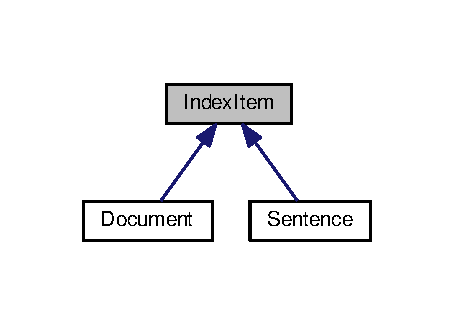
\includegraphics[width=218pt]{classIndexItem__inherit__graph}
\end{center}
\end{figure}
\subsection*{Public Member Functions}
\begin{DoxyCompactItemize}
\item 
\hyperlink{classIndexItem_aa37a5377a9cdd5993b09baad3d842a6f}{Index\+Item} ()
\item 
virtual \hyperlink{classIndexItem_a6225b6cb69e5dc134d2a7cea952cdd17}{$\sim$\+Index\+Item} ()
\item 
const std\+::string \hyperlink{classIndexItem_a269c754227e606efd271bea3e56701f8}{get\+File\+Name} () const
\item 
const std\+::map$<$ const std\+::string, unsigned long $>$ \hyperlink{classIndexItem_a08880ba5d6f18be5b08184df13f37e9f}{get\+Dictionary} () const
\item 
virtual const std\+::size\+\_\+t \hyperlink{classIndexItem_a37bb9320946eedfe8360bc740eb0c11b}{get\+Size} () const
\item 
const std\+::string \hyperlink{classIndexItem_a0cc1631297cb3859a2faecda7062805b}{get\+Content} () const
\item 
const std\+::vector$<$ std\+::string $>$ \hyperlink{classIndexItem_ae37a9af94cfcc8f76fd3081b8096b31a}{get\+Tokens} () const
\end{DoxyCompactItemize}
\subsection*{Protected Attributes}
\begin{DoxyCompactItemize}
\item 
\mbox{\Hypertarget{classIndexItem_a67e954645b9cd94b033c09dc9734b5ea}\label{classIndexItem_a67e954645b9cd94b033c09dc9734b5ea}} 
std\+::string {\bfseries file\+Name}
\item 
\mbox{\Hypertarget{classIndexItem_a259507ae46a62a2411a102b17b731c1f}\label{classIndexItem_a259507ae46a62a2411a102b17b731c1f}} 
std\+::size\+\_\+t {\bfseries size}
\item 
\mbox{\Hypertarget{classIndexItem_a0ff78840db32dd97333a49d69e62ffe6}\label{classIndexItem_a0ff78840db32dd97333a49d69e62ffe6}} 
std\+::string {\bfseries content}
\item 
std\+::vector$<$ std\+::string $>$ \hyperlink{classIndexItem_a36ee76ec7176493ed48952d6231c29f2}{tokens}
\item 
std\+::map$<$ const std\+::string, unsigned long $>$ \hyperlink{classIndexItem_a667ce7eb5e6f22b032dcacd042d89cd3}{dictionary}
\end{DoxyCompactItemize}
\subsection*{Friends}
\begin{DoxyCompactItemize}
\item 
\mbox{\Hypertarget{classIndexItem_acb212461465a08ba81c6b0f35e1151a2}\label{classIndexItem_acb212461465a08ba81c6b0f35e1151a2}} 
std\+::ostream \& {\bfseries operator$<$$<$} (std\+::ostream \&, const \hyperlink{classIndexItem}{Index\+Item} \&)
\end{DoxyCompactItemize}


\subsection{Constructor \& Destructor Documentation}
\mbox{\Hypertarget{classIndexItem_aa37a5377a9cdd5993b09baad3d842a6f}\label{classIndexItem_aa37a5377a9cdd5993b09baad3d842a6f}} 
\index{Index\+Item@{Index\+Item}!Index\+Item@{Index\+Item}}
\index{Index\+Item@{Index\+Item}!Index\+Item@{Index\+Item}}
\subsubsection{\texorpdfstring{Index\+Item()}{IndexItem()}}
{\footnotesize\ttfamily Index\+Item\+::\+Index\+Item (\begin{DoxyParamCaption}{ }\end{DoxyParamCaption})}

Default constructor \mbox{\Hypertarget{classIndexItem_a6225b6cb69e5dc134d2a7cea952cdd17}\label{classIndexItem_a6225b6cb69e5dc134d2a7cea952cdd17}} 
\index{Index\+Item@{Index\+Item}!````~Index\+Item@{$\sim$\+Index\+Item}}
\index{````~Index\+Item@{$\sim$\+Index\+Item}!Index\+Item@{Index\+Item}}
\subsubsection{\texorpdfstring{$\sim$\+Index\+Item()}{~IndexItem()}}
{\footnotesize\ttfamily Index\+Item\+::$\sim$\+Index\+Item (\begin{DoxyParamCaption}{ }\end{DoxyParamCaption})\hspace{0.3cm}{\ttfamily [virtual]}}

Destructor 

\subsection{Member Function Documentation}
\mbox{\Hypertarget{classIndexItem_a0cc1631297cb3859a2faecda7062805b}\label{classIndexItem_a0cc1631297cb3859a2faecda7062805b}} 
\index{Index\+Item@{Index\+Item}!get\+Content@{get\+Content}}
\index{get\+Content@{get\+Content}!Index\+Item@{Index\+Item}}
\subsubsection{\texorpdfstring{get\+Content()}{getContent()}}
{\footnotesize\ttfamily const std\+::string Index\+Item\+::get\+Content (\begin{DoxyParamCaption}{ }\end{DoxyParamCaption}) const}

Get the content of this file \begin{DoxyReturn}{Returns}
the content of this file 
\end{DoxyReturn}
\mbox{\Hypertarget{classIndexItem_a08880ba5d6f18be5b08184df13f37e9f}\label{classIndexItem_a08880ba5d6f18be5b08184df13f37e9f}} 
\index{Index\+Item@{Index\+Item}!get\+Dictionary@{get\+Dictionary}}
\index{get\+Dictionary@{get\+Dictionary}!Index\+Item@{Index\+Item}}
\subsubsection{\texorpdfstring{get\+Dictionary()}{getDictionary()}}
{\footnotesize\ttfamily const std\+::map$<$ const std\+::string, unsigned long $>$ Index\+Item\+::get\+Dictionary (\begin{DoxyParamCaption}{ }\end{DoxyParamCaption}) const}

Get the dictionary map \begin{DoxyReturn}{Returns}

\end{DoxyReturn}
\mbox{\Hypertarget{classIndexItem_a269c754227e606efd271bea3e56701f8}\label{classIndexItem_a269c754227e606efd271bea3e56701f8}} 
\index{Index\+Item@{Index\+Item}!get\+File\+Name@{get\+File\+Name}}
\index{get\+File\+Name@{get\+File\+Name}!Index\+Item@{Index\+Item}}
\subsubsection{\texorpdfstring{get\+File\+Name()}{getFileName()}}
{\footnotesize\ttfamily const std\+::string Index\+Item\+::get\+File\+Name (\begin{DoxyParamCaption}{ }\end{DoxyParamCaption}) const}

Get file name \begin{DoxyReturn}{Returns}
the value of file name 
\end{DoxyReturn}
\mbox{\Hypertarget{classIndexItem_a37bb9320946eedfe8360bc740eb0c11b}\label{classIndexItem_a37bb9320946eedfe8360bc740eb0c11b}} 
\index{Index\+Item@{Index\+Item}!get\+Size@{get\+Size}}
\index{get\+Size@{get\+Size}!Index\+Item@{Index\+Item}}
\subsubsection{\texorpdfstring{get\+Size()}{getSize()}}
{\footnotesize\ttfamily const std\+::size\+\_\+t Index\+Item\+::get\+Size (\begin{DoxyParamCaption}{ }\end{DoxyParamCaption}) const\hspace{0.3cm}{\ttfamily [virtual]}}

Get the size of this file \begin{DoxyReturn}{Returns}
the size in characters of this file 
\end{DoxyReturn}


Reimplemented in \hyperlink{classDocument_a81ccfd6f3de713047ccb52a45842dc26}{Document}, and \hyperlink{classSentence_a2f55ca4244f2ee9c1762019b37734330}{Sentence}.

\mbox{\Hypertarget{classIndexItem_ae37a9af94cfcc8f76fd3081b8096b31a}\label{classIndexItem_ae37a9af94cfcc8f76fd3081b8096b31a}} 
\index{Index\+Item@{Index\+Item}!get\+Tokens@{get\+Tokens}}
\index{get\+Tokens@{get\+Tokens}!Index\+Item@{Index\+Item}}
\subsubsection{\texorpdfstring{get\+Tokens()}{getTokens()}}
{\footnotesize\ttfamily const std\+::vector$<$ std\+::string $>$ Index\+Item\+::get\+Tokens (\begin{DoxyParamCaption}{ }\end{DoxyParamCaption}) const}

Get tokens \begin{DoxyReturn}{Returns}

\end{DoxyReturn}


\subsection{Member Data Documentation}
\mbox{\Hypertarget{classIndexItem_a667ce7eb5e6f22b032dcacd042d89cd3}\label{classIndexItem_a667ce7eb5e6f22b032dcacd042d89cd3}} 
\index{Index\+Item@{Index\+Item}!dictionary@{dictionary}}
\index{dictionary@{dictionary}!Index\+Item@{Index\+Item}}
\subsubsection{\texorpdfstring{dictionary}{dictionary}}
{\footnotesize\ttfamily std\+::map$<$const std\+::string, unsigned long$>$ Index\+Item\+::dictionary\hspace{0.3cm}{\ttfamily [protected]}}

word and word count in the index\+Item \mbox{\Hypertarget{classIndexItem_a36ee76ec7176493ed48952d6231c29f2}\label{classIndexItem_a36ee76ec7176493ed48952d6231c29f2}} 
\index{Index\+Item@{Index\+Item}!tokens@{tokens}}
\index{tokens@{tokens}!Index\+Item@{Index\+Item}}
\subsubsection{\texorpdfstring{tokens}{tokens}}
{\footnotesize\ttfamily std\+::vector$<$std\+::string$>$ Index\+Item\+::tokens\hspace{0.3cm}{\ttfamily [protected]}}

words in the index\+Item 

The documentation for this class was generated from the following files\+:\begin{DoxyCompactItemize}
\item 
headers/Index\+Item.\+h\item 
implementation/Index\+Item.\+cpp\end{DoxyCompactItemize}

\hypertarget{classQueryResult}{}\section{Query\+Result Class Reference}
\label{classQueryResult}\index{Query\+Result@{Query\+Result}}


{\ttfamily \#include $<$Query\+Result.\+h$>$}



Collaboration diagram for Query\+Result\+:\nopagebreak
\begin{figure}[H]
\begin{center}
\leavevmode
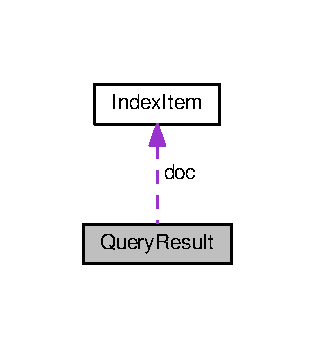
\includegraphics[width=151pt]{classQueryResult__coll__graph}
\end{center}
\end{figure}
\subsection*{Public Member Functions}
\begin{DoxyCompactItemize}
\item 
\hyperlink{classQueryResult_a23c0f8433d60025e81759f569dc08ab8}{Query\+Result} ()
\item 
\hyperlink{classQueryResult_ae765defee1fe2d3a1361f00d24de6f8b}{Query\+Result} (const \hyperlink{classIndexItem}{Index\+Item} \hyperlink{classQueryResult_ab078a6cc489f8f8f05d7ea97d8514b82}{doc}, const double \hyperlink{classQueryResult_ab76d940559daeac2b7eace3851c9a162}{score})
\end{DoxyCompactItemize}
\subsection*{Public Attributes}
\begin{DoxyCompactItemize}
\item 
const \hyperlink{classIndexItem}{Index\+Item} \hyperlink{classQueryResult_ab078a6cc489f8f8f05d7ea97d8514b82}{doc}
\item 
const double \hyperlink{classQueryResult_ab76d940559daeac2b7eace3851c9a162}{score}
\end{DoxyCompactItemize}
\subsection*{Friends}
\begin{DoxyCompactItemize}
\item 
\mbox{\Hypertarget{classQueryResult_a508480dcd37309a0df1c62221b6a15e3}\label{classQueryResult_a508480dcd37309a0df1c62221b6a15e3}} 
std\+::ostream \& {\bfseries operator$<$$<$} (std\+::ostream \&, const \hyperlink{classQueryResult}{Query\+Result} \&)
\end{DoxyCompactItemize}


\subsection{Detailed Description}
Storing the document and the score information for the query word 

\subsection{Constructor \& Destructor Documentation}
\mbox{\Hypertarget{classQueryResult_a23c0f8433d60025e81759f569dc08ab8}\label{classQueryResult_a23c0f8433d60025e81759f569dc08ab8}} 
\index{Query\+Result@{Query\+Result}!Query\+Result@{Query\+Result}}
\index{Query\+Result@{Query\+Result}!Query\+Result@{Query\+Result}}
\subsubsection{\texorpdfstring{Query\+Result()}{QueryResult()}\hspace{0.1cm}{\footnotesize\ttfamily [1/2]}}
{\footnotesize\ttfamily Query\+Result\+::\+Query\+Result (\begin{DoxyParamCaption}{ }\end{DoxyParamCaption})}

Default constructor \mbox{\Hypertarget{classQueryResult_ae765defee1fe2d3a1361f00d24de6f8b}\label{classQueryResult_ae765defee1fe2d3a1361f00d24de6f8b}} 
\index{Query\+Result@{Query\+Result}!Query\+Result@{Query\+Result}}
\index{Query\+Result@{Query\+Result}!Query\+Result@{Query\+Result}}
\subsubsection{\texorpdfstring{Query\+Result()}{QueryResult()}\hspace{0.1cm}{\footnotesize\ttfamily [2/2]}}
{\footnotesize\ttfamily Query\+Result\+::\+Query\+Result (\begin{DoxyParamCaption}\item[{const \hyperlink{classIndexItem}{Index\+Item}}]{doc,  }\item[{const double}]{score }\end{DoxyParamCaption})}

Constructor accepting a \hyperlink{classIndexItem}{Index\+Item} and its score 
\begin{DoxyParams}{Parameters}
{\em doc} & \\
\hline
{\em score} & \\
\hline
\end{DoxyParams}


\subsection{Member Data Documentation}
\mbox{\Hypertarget{classQueryResult_ab078a6cc489f8f8f05d7ea97d8514b82}\label{classQueryResult_ab078a6cc489f8f8f05d7ea97d8514b82}} 
\index{Query\+Result@{Query\+Result}!doc@{doc}}
\index{doc@{doc}!Query\+Result@{Query\+Result}}
\subsubsection{\texorpdfstring{doc}{doc}}
{\footnotesize\ttfamily const \hyperlink{classIndexItem}{Index\+Item} Query\+Result\+::doc}

the current document in the query result. \mbox{\Hypertarget{classQueryResult_ab76d940559daeac2b7eace3851c9a162}\label{classQueryResult_ab76d940559daeac2b7eace3851c9a162}} 
\index{Query\+Result@{Query\+Result}!score@{score}}
\index{score@{score}!Query\+Result@{Query\+Result}}
\subsubsection{\texorpdfstring{score}{score}}
{\footnotesize\ttfamily const double Query\+Result\+::score}

the score related to this document 

The documentation for this class was generated from the following files\+:\begin{DoxyCompactItemize}
\item 
headers/Query\+Result.\+h\item 
implementation/Query\+Result.\+cpp\end{DoxyCompactItemize}

\hypertarget{classSentence}{}\section{Sentence Class Reference}
\label{classSentence}\index{Sentence@{Sentence}}


Inheritance diagram for Sentence\+:\nopagebreak
\begin{figure}[H]
\begin{center}
\leavevmode
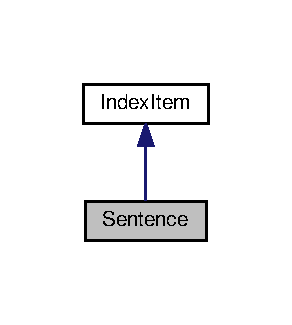
\includegraphics[width=140pt]{classSentence__inherit__graph}
\end{center}
\end{figure}


Collaboration diagram for Sentence\+:\nopagebreak
\begin{figure}[H]
\begin{center}
\leavevmode
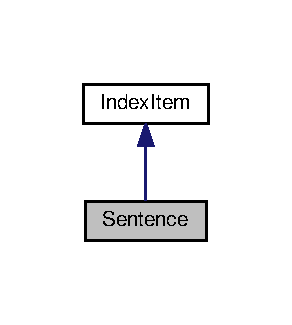
\includegraphics[width=140pt]{classSentence__coll__graph}
\end{center}
\end{figure}
\subsection*{Public Member Functions}
\begin{DoxyCompactItemize}
\item 
\hyperlink{classSentence_aa767c3de8aaf7f2e30fa7524cdfcaead}{Sentence} ()
\item 
\hyperlink{classSentence_a92557fe647ad458e02749286b71f2586}{Sentence} (const std\+::string \&name)
\item 
const std\+::size\+\_\+t \hyperlink{classSentence_a2f55ca4244f2ee9c1762019b37734330}{get\+Size} () const override final
\item 
const std\+::size\+\_\+t \hyperlink{classSentence_ab3d1877176dc98185753ee23a0897c1d}{get\+Pos} (const std\+::string \&) const
\end{DoxyCompactItemize}
\subsection*{Friends}
\begin{DoxyCompactItemize}
\item 
\mbox{\Hypertarget{classSentence_ab4f19f42171de5744a04fed46ecbcc63}\label{classSentence_ab4f19f42171de5744a04fed46ecbcc63}} 
std\+::ostream \& {\bfseries operator$<$$<$} (std\+::ostream \&, const \hyperlink{classSentence}{Sentence} \&)
\end{DoxyCompactItemize}
\subsection*{Additional Inherited Members}


\subsection{Constructor \& Destructor Documentation}
\mbox{\Hypertarget{classSentence_aa767c3de8aaf7f2e30fa7524cdfcaead}\label{classSentence_aa767c3de8aaf7f2e30fa7524cdfcaead}} 
\index{Sentence@{Sentence}!Sentence@{Sentence}}
\index{Sentence@{Sentence}!Sentence@{Sentence}}
\subsubsection{\texorpdfstring{Sentence()}{Sentence()}\hspace{0.1cm}{\footnotesize\ttfamily [1/2]}}
{\footnotesize\ttfamily Sentence\+::\+Sentence (\begin{DoxyParamCaption}{ }\end{DoxyParamCaption})}

Default constructor \mbox{\Hypertarget{classSentence_a92557fe647ad458e02749286b71f2586}\label{classSentence_a92557fe647ad458e02749286b71f2586}} 
\index{Sentence@{Sentence}!Sentence@{Sentence}}
\index{Sentence@{Sentence}!Sentence@{Sentence}}
\subsubsection{\texorpdfstring{Sentence()}{Sentence()}\hspace{0.1cm}{\footnotesize\ttfamily [2/2]}}
{\footnotesize\ttfamily Sentence\+::\+Sentence (\begin{DoxyParamCaption}\item[{const std\+::string \&}]{name }\end{DoxyParamCaption})}

Constructor accepts a string 
\begin{DoxyParams}{Parameters}
{\em str} & \\
\hline
\end{DoxyParams}


\subsection{Member Function Documentation}
\mbox{\Hypertarget{classSentence_ab3d1877176dc98185753ee23a0897c1d}\label{classSentence_ab3d1877176dc98185753ee23a0897c1d}} 
\index{Sentence@{Sentence}!get\+Pos@{get\+Pos}}
\index{get\+Pos@{get\+Pos}!Sentence@{Sentence}}
\subsubsection{\texorpdfstring{get\+Pos()}{getPos()}}
{\footnotesize\ttfamily const size\+\_\+t Sentence\+::get\+Pos (\begin{DoxyParamCaption}\item[{const std\+::string \&}]{sen }\end{DoxyParamCaption}) const}

Get the position of the sentence in the document \begin{DoxyReturn}{Returns}

\end{DoxyReturn}
\mbox{\Hypertarget{classSentence_a2f55ca4244f2ee9c1762019b37734330}\label{classSentence_a2f55ca4244f2ee9c1762019b37734330}} 
\index{Sentence@{Sentence}!get\+Size@{get\+Size}}
\index{get\+Size@{get\+Size}!Sentence@{Sentence}}
\subsubsection{\texorpdfstring{get\+Size()}{getSize()}}
{\footnotesize\ttfamily const size\+\_\+t Sentence\+::get\+Size (\begin{DoxyParamCaption}{ }\end{DoxyParamCaption}) const\hspace{0.3cm}{\ttfamily [final]}, {\ttfamily [override]}, {\ttfamily [virtual]}}

Get document size \begin{DoxyReturn}{Returns}
the size of document 
\end{DoxyReturn}


Reimplemented from \hyperlink{classIndexItem_a37bb9320946eedfe8360bc740eb0c11b}{Index\+Item}.



The documentation for this class was generated from the following files\+:\begin{DoxyCompactItemize}
\item 
headers/Sentence.\+h\item 
implementation/Sentence.\+cpp\end{DoxyCompactItemize}

\hypertarget{classSentenceIndexer}{}\section{Sentence\+Indexer Class Reference}
\label{classSentenceIndexer}\index{Sentence\+Indexer@{Sentence\+Indexer}}


Inheritance diagram for Sentence\+Indexer\+:\nopagebreak
\begin{figure}[H]
\begin{center}
\leavevmode
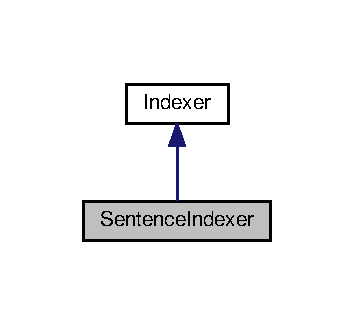
\includegraphics[width=170pt]{classSentenceIndexer__inherit__graph}
\end{center}
\end{figure}


Collaboration diagram for Sentence\+Indexer\+:\nopagebreak
\begin{figure}[H]
\begin{center}
\leavevmode
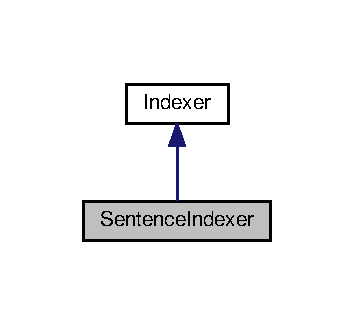
\includegraphics[width=170pt]{classSentenceIndexer__coll__graph}
\end{center}
\end{figure}
\subsection*{Public Member Functions}
\begin{DoxyCompactItemize}
\item 
\hyperlink{classSentenceIndexer_a2ec9f359954191ebc5d84c759fd2238d}{Sentence\+Indexer} ()
\item 
\hyperlink{classSentenceIndexer_a3402eb910551128d0c8ecb33cf0bae42}{$\sim$\+Sentence\+Indexer} ()
\item 
virtual const std\+::vector$<$ \hyperlink{classQueryResult}{Query\+Result} $>$ \hyperlink{classSentenceIndexer_ac9b17bde40b851d8e0c263ce2241b9c4}{query} (const std\+::string, const unsigned int=500) override
\item 
virtual const \hyperlink{classIndexItem}{Index\+Item} \& \hyperlink{classSentenceIndexer_a0c0b7ee70c1d183e6bd6ca4ee412831c}{operator\mbox{[}$\,$\mbox{]}} (unsigned long) const override
\end{DoxyCompactItemize}
\subsection*{Friends}
\begin{DoxyCompactItemize}
\item 
\mbox{\Hypertarget{classSentenceIndexer_a28ba47a4a3b51dc012fa2f8fb194ab22}\label{classSentenceIndexer_a28ba47a4a3b51dc012fa2f8fb194ab22}} 
std\+::ostream \& {\bfseries operator$<$$<$} (std\+::ostream \&, const \hyperlink{classSentenceIndexer}{Sentence\+Indexer} \&)
\end{DoxyCompactItemize}
\subsection*{Additional Inherited Members}


\subsection{Constructor \& Destructor Documentation}
\mbox{\Hypertarget{classSentenceIndexer_a2ec9f359954191ebc5d84c759fd2238d}\label{classSentenceIndexer_a2ec9f359954191ebc5d84c759fd2238d}} 
\index{Sentence\+Indexer@{Sentence\+Indexer}!Sentence\+Indexer@{Sentence\+Indexer}}
\index{Sentence\+Indexer@{Sentence\+Indexer}!Sentence\+Indexer@{Sentence\+Indexer}}
\subsubsection{\texorpdfstring{Sentence\+Indexer()}{SentenceIndexer()}}
{\footnotesize\ttfamily Sentence\+Indexer\+::\+Sentence\+Indexer (\begin{DoxyParamCaption}{ }\end{DoxyParamCaption})}

Default constructor \mbox{\Hypertarget{classSentenceIndexer_a3402eb910551128d0c8ecb33cf0bae42}\label{classSentenceIndexer_a3402eb910551128d0c8ecb33cf0bae42}} 
\index{Sentence\+Indexer@{Sentence\+Indexer}!````~Sentence\+Indexer@{$\sim$\+Sentence\+Indexer}}
\index{````~Sentence\+Indexer@{$\sim$\+Sentence\+Indexer}!Sentence\+Indexer@{Sentence\+Indexer}}
\subsubsection{\texorpdfstring{$\sim$\+Sentence\+Indexer()}{~SentenceIndexer()}}
{\footnotesize\ttfamily Sentence\+Indexer\+::$\sim$\+Sentence\+Indexer (\begin{DoxyParamCaption}{ }\end{DoxyParamCaption})\hspace{0.3cm}{\ttfamily [inline]}}

Default destructor 

\subsection{Member Function Documentation}
\mbox{\Hypertarget{classSentenceIndexer_a0c0b7ee70c1d183e6bd6ca4ee412831c}\label{classSentenceIndexer_a0c0b7ee70c1d183e6bd6ca4ee412831c}} 
\index{Sentence\+Indexer@{Sentence\+Indexer}!operator\mbox{[}\mbox{]}@{operator[]}}
\index{operator\mbox{[}\mbox{]}@{operator[]}!Sentence\+Indexer@{Sentence\+Indexer}}
\subsubsection{\texorpdfstring{operator[]()}{operator[]()}}
{\footnotesize\ttfamily const \hyperlink{classIndexItem}{Index\+Item} \& Sentence\+Indexer\+::operator\mbox{[}$\,$\mbox{]} (\begin{DoxyParamCaption}\item[{unsigned long}]{index }\end{DoxyParamCaption}) const\hspace{0.3cm}{\ttfamily [override]}, {\ttfamily [virtual]}}

Get the index\+Item at given position \begin{DoxyReturn}{Returns}

\end{DoxyReturn}


Reimplemented from \hyperlink{classIndexer_ac9a2012415a2b06251852047e30bf618}{Indexer}.

\mbox{\Hypertarget{classSentenceIndexer_ac9b17bde40b851d8e0c263ce2241b9c4}\label{classSentenceIndexer_ac9b17bde40b851d8e0c263ce2241b9c4}} 
\index{Sentence\+Indexer@{Sentence\+Indexer}!query@{query}}
\index{query@{query}!Sentence\+Indexer@{Sentence\+Indexer}}
\subsubsection{\texorpdfstring{query()}{query()}}
{\footnotesize\ttfamily const vector$<$ \hyperlink{classQueryResult}{Query\+Result} $>$ Sentence\+Indexer\+::query (\begin{DoxyParamCaption}\item[{const std\+::string}]{s,  }\item[{const unsigned int}]{top = {\ttfamily 500} }\end{DoxyParamCaption})\hspace{0.3cm}{\ttfamily [override]}, {\ttfamily [virtual]}}

Query by giving string \begin{DoxyReturn}{Returns}

\end{DoxyReturn}


Reimplemented from \hyperlink{classIndexer_abd1dd6a6da0c9e43efaa99866c538e6c}{Indexer}.



The documentation for this class was generated from the following files\+:\begin{DoxyCompactItemize}
\item 
headers/Sentence\+Indexer.\+h\item 
implementation/Sentence\+Indexer.\+cpp\end{DoxyCompactItemize}

\hypertarget{classSentenceTokenizer}{\section{Sentence\-Tokenizer Class Reference}
\label{classSentenceTokenizer}\index{Sentence\-Tokenizer@{Sentence\-Tokenizer}}
}
Inheritance diagram for Sentence\-Tokenizer\-:\begin{figure}[H]
\begin{center}
\leavevmode
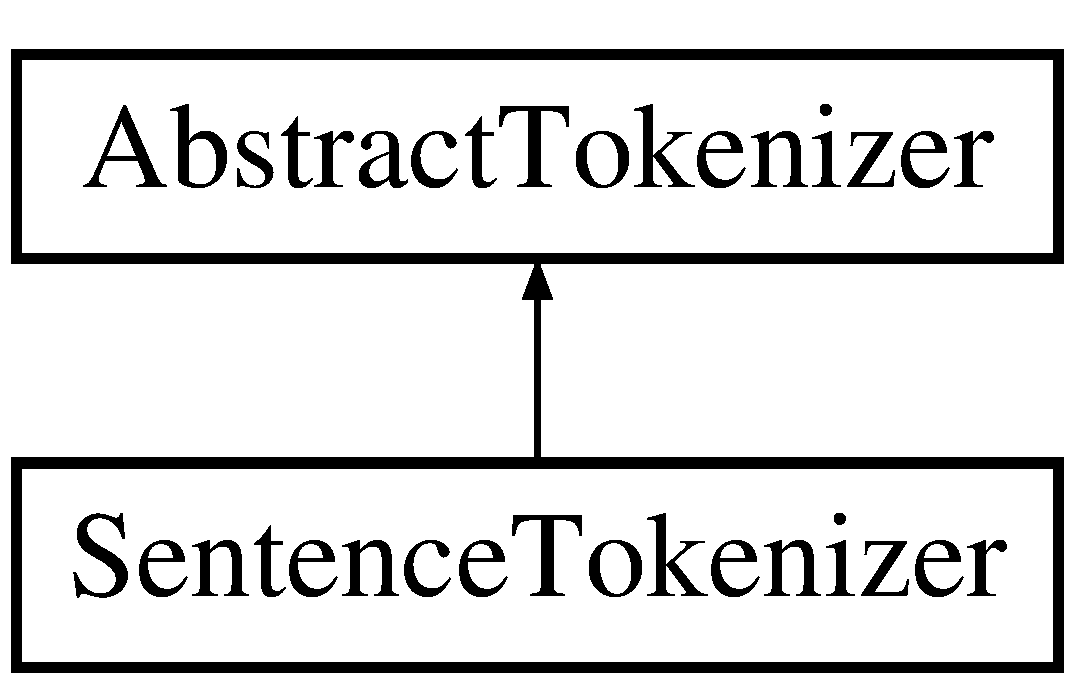
\includegraphics[height=2.000000cm]{classSentenceTokenizer}
\end{center}
\end{figure}
\subsection*{Public Member Functions}
\begin{DoxyCompactItemize}
\item 
\hyperlink{classSentenceTokenizer_a7ac4c0f31e4066808cb2f4e8f1aee545}{Sentence\-Tokenizer} ()
\item 
\hyperlink{classSentenceTokenizer_a3ac263cb539f5dd072931a4d9f134d74}{Sentence\-Tokenizer} (const std\-::string \&input\-String)
\item 
virtual \hyperlink{classSentenceTokenizer_a91bcdff9ff84fce9c56208c19254bdba}{$\sim$\-Sentence\-Tokenizer} ()
\end{DoxyCompactItemize}
\subsection*{Friends}
\begin{DoxyCompactItemize}
\item 
\hypertarget{classSentenceTokenizer_a2998282df2f8bc7eb4c49617879f9256}{std\-::ostream \& {\bfseries operator$<$$<$} (std\-::ostream \&, const \hyperlink{classSentenceTokenizer}{Sentence\-Tokenizer} \&)}\label{classSentenceTokenizer_a2998282df2f8bc7eb4c49617879f9256}

\end{DoxyCompactItemize}
\subsection*{Additional Inherited Members}


\subsection{Constructor \& Destructor Documentation}
\hypertarget{classSentenceTokenizer_a7ac4c0f31e4066808cb2f4e8f1aee545}{\index{Sentence\-Tokenizer@{Sentence\-Tokenizer}!Sentence\-Tokenizer@{Sentence\-Tokenizer}}
\index{Sentence\-Tokenizer@{Sentence\-Tokenizer}!SentenceTokenizer@{Sentence\-Tokenizer}}
\subsubsection[{Sentence\-Tokenizer}]{\setlength{\rightskip}{0pt plus 5cm}Sentence\-Tokenizer\-::\-Sentence\-Tokenizer (
\begin{DoxyParamCaption}
{}
\end{DoxyParamCaption}
)}}\label{classSentenceTokenizer_a7ac4c0f31e4066808cb2f4e8f1aee545}
Default constructor \hypertarget{classSentenceTokenizer_a3ac263cb539f5dd072931a4d9f134d74}{\index{Sentence\-Tokenizer@{Sentence\-Tokenizer}!Sentence\-Tokenizer@{Sentence\-Tokenizer}}
\index{Sentence\-Tokenizer@{Sentence\-Tokenizer}!SentenceTokenizer@{Sentence\-Tokenizer}}
\subsubsection[{Sentence\-Tokenizer}]{\setlength{\rightskip}{0pt plus 5cm}Sentence\-Tokenizer\-::\-Sentence\-Tokenizer (
\begin{DoxyParamCaption}
\item[{const std\-::string \&}]{input\-String}
\end{DoxyParamCaption}
)}}\label{classSentenceTokenizer_a3ac263cb539f5dd072931a4d9f134d74}
Tokenizer a file by accepting a file name \hypertarget{classSentenceTokenizer_a91bcdff9ff84fce9c56208c19254bdba}{\index{Sentence\-Tokenizer@{Sentence\-Tokenizer}!$\sim$\-Sentence\-Tokenizer@{$\sim$\-Sentence\-Tokenizer}}
\index{$\sim$\-Sentence\-Tokenizer@{$\sim$\-Sentence\-Tokenizer}!SentenceTokenizer@{Sentence\-Tokenizer}}
\subsubsection[{$\sim$\-Sentence\-Tokenizer}]{\setlength{\rightskip}{0pt plus 5cm}virtual Sentence\-Tokenizer\-::$\sim$\-Sentence\-Tokenizer (
\begin{DoxyParamCaption}
{}
\end{DoxyParamCaption}
)\hspace{0.3cm}{\ttfamily [inline]}, {\ttfamily [virtual]}}}\label{classSentenceTokenizer_a91bcdff9ff84fce9c56208c19254bdba}
Default destructor 

The documentation for this class was generated from the following files\-:\begin{DoxyCompactItemize}
\item 
headers/Sentence\-Tokenizer.\-h\item 
implementation/Sentence\-Tokenizer.\-cpp\end{DoxyCompactItemize}

\hypertarget{classStopword}{\section{Stopword Class Reference}
\label{classStopword}\index{Stopword@{Stopword}}
}


{\ttfamily \#include $<$Stopword.\-h$>$}

\subsection*{Public Member Functions}
\begin{DoxyCompactItemize}
\item 
\hyperlink{classStopword_a9580930ded0ee601ad610a078914a628}{Stopword} ()
\item 
\hyperlink{classStopword_a7905aacd5d59b997b50506a71d12a0f7}{Stopword} (const std\-::string \&file)
\item 
bool \hyperlink{classStopword_a2acde54983583632735c84fdb0c12d7e}{operator()} (const std\-::string \&)
\item 
const std\-::vector$<$ std\-::string $>$ \& \hyperlink{classStopword_a1b84b6472d0cbf2886f9d5a9b235b0d0}{get\-Stop\-Words} () const 
\end{DoxyCompactItemize}
\subsection*{Friends}
\begin{DoxyCompactItemize}
\item 
\hypertarget{classStopword_a33de0e6203154212a6d2f798efd40d67}{std\-::ostream \& {\bfseries operator$<$$<$} (std\-::ostream \&, const \hyperlink{classStopword}{Stopword} \&)}\label{classStopword_a33de0e6203154212a6d2f798efd40d67}

\end{DoxyCompactItemize}


\subsection{Detailed Description}
the words not to be showing in the output 

\subsection{Constructor \& Destructor Documentation}
\hypertarget{classStopword_a9580930ded0ee601ad610a078914a628}{\index{Stopword@{Stopword}!Stopword@{Stopword}}
\index{Stopword@{Stopword}!Stopword@{Stopword}}
\subsubsection[{Stopword}]{\setlength{\rightskip}{0pt plus 5cm}Stopword\-::\-Stopword (
\begin{DoxyParamCaption}
{}
\end{DoxyParamCaption}
)}}\label{classStopword_a9580930ded0ee601ad610a078914a628}
Default constructor \hypertarget{classStopword_a7905aacd5d59b997b50506a71d12a0f7}{\index{Stopword@{Stopword}!Stopword@{Stopword}}
\index{Stopword@{Stopword}!Stopword@{Stopword}}
\subsubsection[{Stopword}]{\setlength{\rightskip}{0pt plus 5cm}Stopword\-::\-Stopword (
\begin{DoxyParamCaption}
\item[{const std\-::string \&}]{file}
\end{DoxyParamCaption}
)}}\label{classStopword_a7905aacd5d59b997b50506a71d12a0f7}
Constructor accepts a string 

\subsection{Member Function Documentation}
\hypertarget{classStopword_a1b84b6472d0cbf2886f9d5a9b235b0d0}{\index{Stopword@{Stopword}!get\-Stop\-Words@{get\-Stop\-Words}}
\index{get\-Stop\-Words@{get\-Stop\-Words}!Stopword@{Stopword}}
\subsubsection[{get\-Stop\-Words}]{\setlength{\rightskip}{0pt plus 5cm}const vector$<$ string $>$ \& Stopword\-::get\-Stop\-Words (
\begin{DoxyParamCaption}
{}
\end{DoxyParamCaption}
) const}}\label{classStopword_a1b84b6472d0cbf2886f9d5a9b235b0d0}
Get stop words \begin{DoxyReturn}{Returns}

\end{DoxyReturn}
\hypertarget{classStopword_a2acde54983583632735c84fdb0c12d7e}{\index{Stopword@{Stopword}!operator()@{operator()}}
\index{operator()@{operator()}!Stopword@{Stopword}}
\subsubsection[{operator()}]{\setlength{\rightskip}{0pt plus 5cm}bool Stopword\-::operator() (
\begin{DoxyParamCaption}
\item[{const std\-::string \&}]{}
\end{DoxyParamCaption}
)}}\label{classStopword_a2acde54983583632735c84fdb0c12d7e}
Overload () \begin{DoxyReturn}{Returns}

\end{DoxyReturn}


The documentation for this class was generated from the following files\-:\begin{DoxyCompactItemize}
\item 
headers/Stopword.\-h\item 
implementation/Stopword.\-cpp\end{DoxyCompactItemize}

\hypertarget{classWordTokenizer}{}\section{Word\+Tokenizer Class Reference}
\label{classWordTokenizer}\index{Word\+Tokenizer@{Word\+Tokenizer}}


Inheritance diagram for Word\+Tokenizer\+:\nopagebreak
\begin{figure}[H]
\begin{center}
\leavevmode
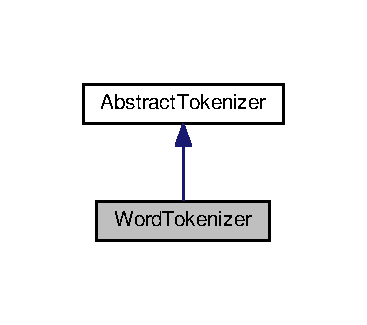
\includegraphics[width=176pt]{classWordTokenizer__inherit__graph}
\end{center}
\end{figure}


Collaboration diagram for Word\+Tokenizer\+:\nopagebreak
\begin{figure}[H]
\begin{center}
\leavevmode
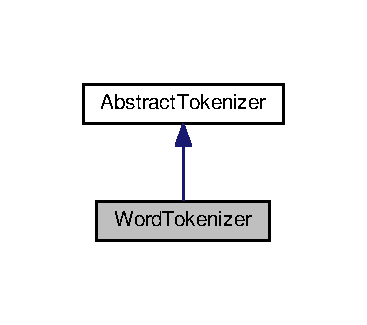
\includegraphics[width=176pt]{classWordTokenizer__coll__graph}
\end{center}
\end{figure}
\subsection*{Public Member Functions}
\begin{DoxyCompactItemize}
\item 
\hyperlink{classWordTokenizer_a78cfc8455e2b0d99ae070a9d9ef647c8}{Word\+Tokenizer} ()
\item 
\hyperlink{classWordTokenizer_ab360e49e4fc162e48060c0811d4d19f8}{Word\+Tokenizer} (const std\+::string \&input\+String)
\item 
virtual \hyperlink{classWordTokenizer_a04c986b8527bd4f556443161804b1208}{$\sim$\+Word\+Tokenizer} ()
\end{DoxyCompactItemize}
\subsection*{Friends}
\begin{DoxyCompactItemize}
\item 
\mbox{\Hypertarget{classWordTokenizer_aa4996c7e6f7338a26da11ab4a0f15b78}\label{classWordTokenizer_aa4996c7e6f7338a26da11ab4a0f15b78}} 
std\+::ostream \& {\bfseries operator$<$$<$} (std\+::ostream \&, const \hyperlink{classWordTokenizer}{Word\+Tokenizer} \&)
\end{DoxyCompactItemize}
\subsection*{Additional Inherited Members}


\subsection{Constructor \& Destructor Documentation}
\mbox{\Hypertarget{classWordTokenizer_a78cfc8455e2b0d99ae070a9d9ef647c8}\label{classWordTokenizer_a78cfc8455e2b0d99ae070a9d9ef647c8}} 
\index{Word\+Tokenizer@{Word\+Tokenizer}!Word\+Tokenizer@{Word\+Tokenizer}}
\index{Word\+Tokenizer@{Word\+Tokenizer}!Word\+Tokenizer@{Word\+Tokenizer}}
\subsubsection{\texorpdfstring{Word\+Tokenizer()}{WordTokenizer()}\hspace{0.1cm}{\footnotesize\ttfamily [1/2]}}
{\footnotesize\ttfamily Word\+Tokenizer\+::\+Word\+Tokenizer (\begin{DoxyParamCaption}{ }\end{DoxyParamCaption})}

Default constructor \mbox{\Hypertarget{classWordTokenizer_ab360e49e4fc162e48060c0811d4d19f8}\label{classWordTokenizer_ab360e49e4fc162e48060c0811d4d19f8}} 
\index{Word\+Tokenizer@{Word\+Tokenizer}!Word\+Tokenizer@{Word\+Tokenizer}}
\index{Word\+Tokenizer@{Word\+Tokenizer}!Word\+Tokenizer@{Word\+Tokenizer}}
\subsubsection{\texorpdfstring{Word\+Tokenizer()}{WordTokenizer()}\hspace{0.1cm}{\footnotesize\ttfamily [2/2]}}
{\footnotesize\ttfamily Word\+Tokenizer\+::\+Word\+Tokenizer (\begin{DoxyParamCaption}\item[{const std\+::string \&}]{input\+String }\end{DoxyParamCaption})}

Constructor accepting a file name 
\begin{DoxyParams}{Parameters}
{\em input\+String} & \\
\hline
\end{DoxyParams}
\mbox{\Hypertarget{classWordTokenizer_a04c986b8527bd4f556443161804b1208}\label{classWordTokenizer_a04c986b8527bd4f556443161804b1208}} 
\index{Word\+Tokenizer@{Word\+Tokenizer}!````~Word\+Tokenizer@{$\sim$\+Word\+Tokenizer}}
\index{````~Word\+Tokenizer@{$\sim$\+Word\+Tokenizer}!Word\+Tokenizer@{Word\+Tokenizer}}
\subsubsection{\texorpdfstring{$\sim$\+Word\+Tokenizer()}{~WordTokenizer()}}
{\footnotesize\ttfamily virtual Word\+Tokenizer\+::$\sim$\+Word\+Tokenizer (\begin{DoxyParamCaption}{ }\end{DoxyParamCaption})\hspace{0.3cm}{\ttfamily [inline]}, {\ttfamily [virtual]}}

Default destructor 

The documentation for this class was generated from the following files\+:\begin{DoxyCompactItemize}
\item 
headers/Word\+Tokenizer.\+h\item 
implementation/Word\+Tokenizer.\+cpp\end{DoxyCompactItemize}

%--- End generated contents ---

% Index
\backmatter
\newpage
\phantomsection
\clearemptydoublepage
\addcontentsline{toc}{chapter}{Index}
\printindex

\end{document}
